\documentclass{beamer}
\usetheme{Antibes}

\usepackage[makeroom]{cancel}
\usepackage{graphicx}

\def\*#1{\mathbf{#1}}
\def\rr{\rightarrow}
\newcommand{\norm}[1]{\left\lVert#1\right\rVert}
\usefonttheme[onlymath]{serif}

\title[curvature]{Discrete Curvature Computation\\ \small{Work Report}}
\author{MinliangLIN}
\date{\tiny\today}

\begin{document}
\frame{\titlepage}

\begin{frame}
  \frametitle{Outline}
  \tableofcontents
\end{frame}

\section{fxzlib of curvature}
\frame{{What is curvature?}
\begin{itemize}
  \item A number indicating how blend a curve is, which lays on surface
  \item How fast does a curve leave the tagent plane?
\end{itemize}
  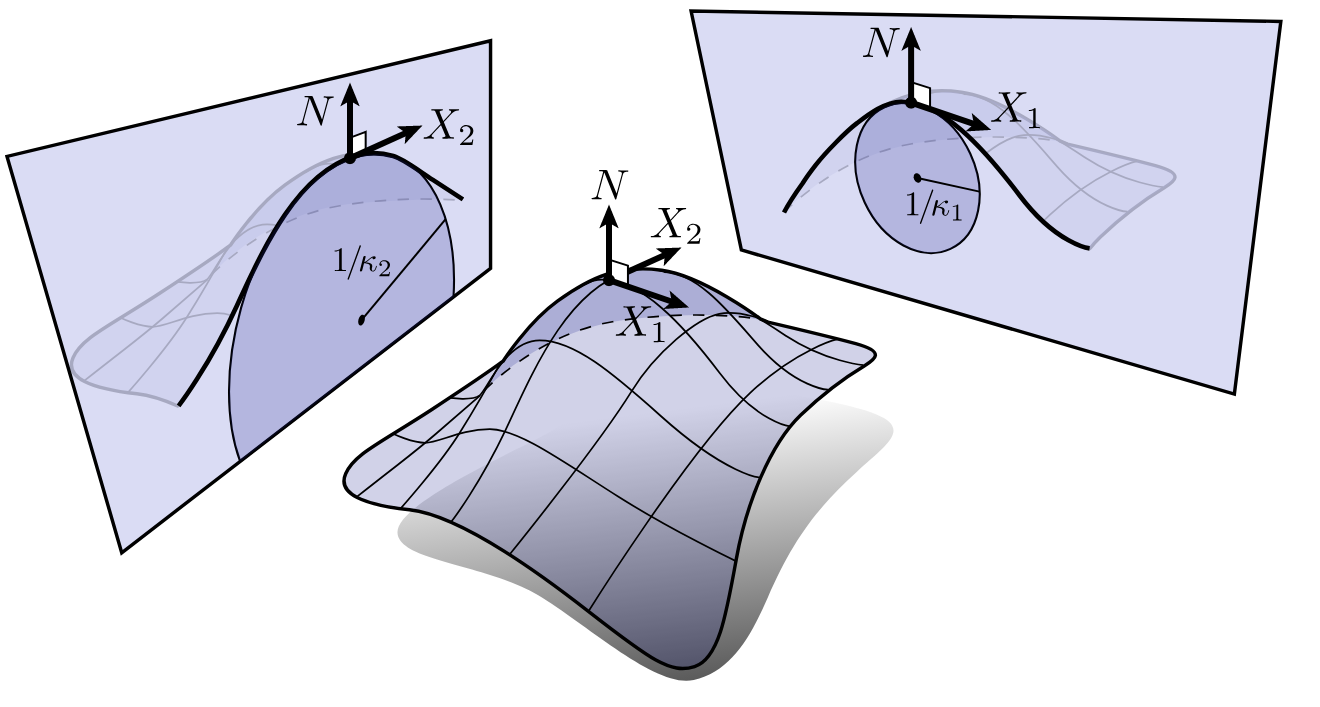
\includegraphics[width=0.7\textwidth]{img/principal}
}

\frame{{Motivation}
controlling the direction and size of quadrangulation
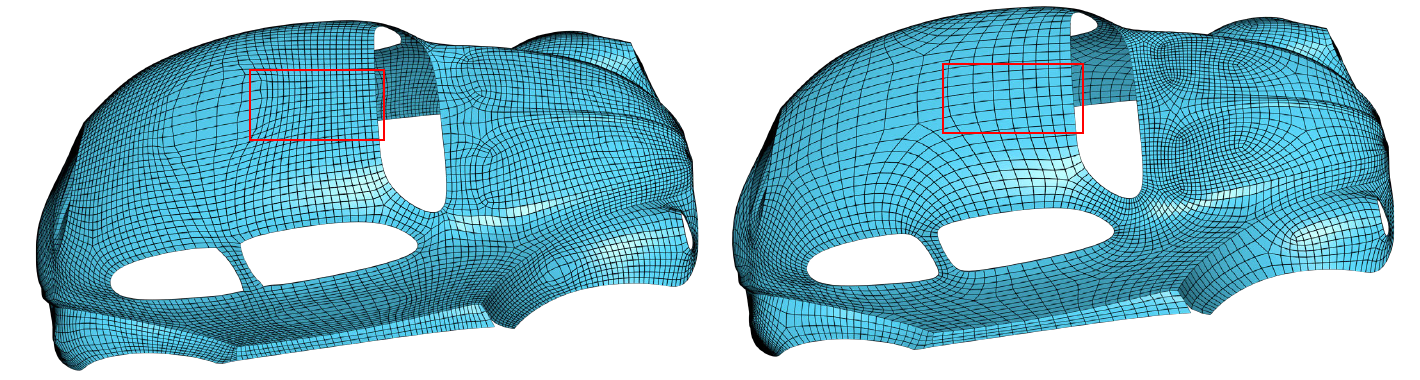
\includegraphics[width=\textwidth]{img/car}
}

\frame{{What is curvature}
\begin{itemize}
  \item<1-> A quadratic form of tagent vector $X^TBX$
  \item<2-> $B$ is a \textbf{linear map / tensor} from $dX$ to $dN$
  \item<3-> mean curvature $\kappa_H = tr(B)/2$
\end{itemize}
  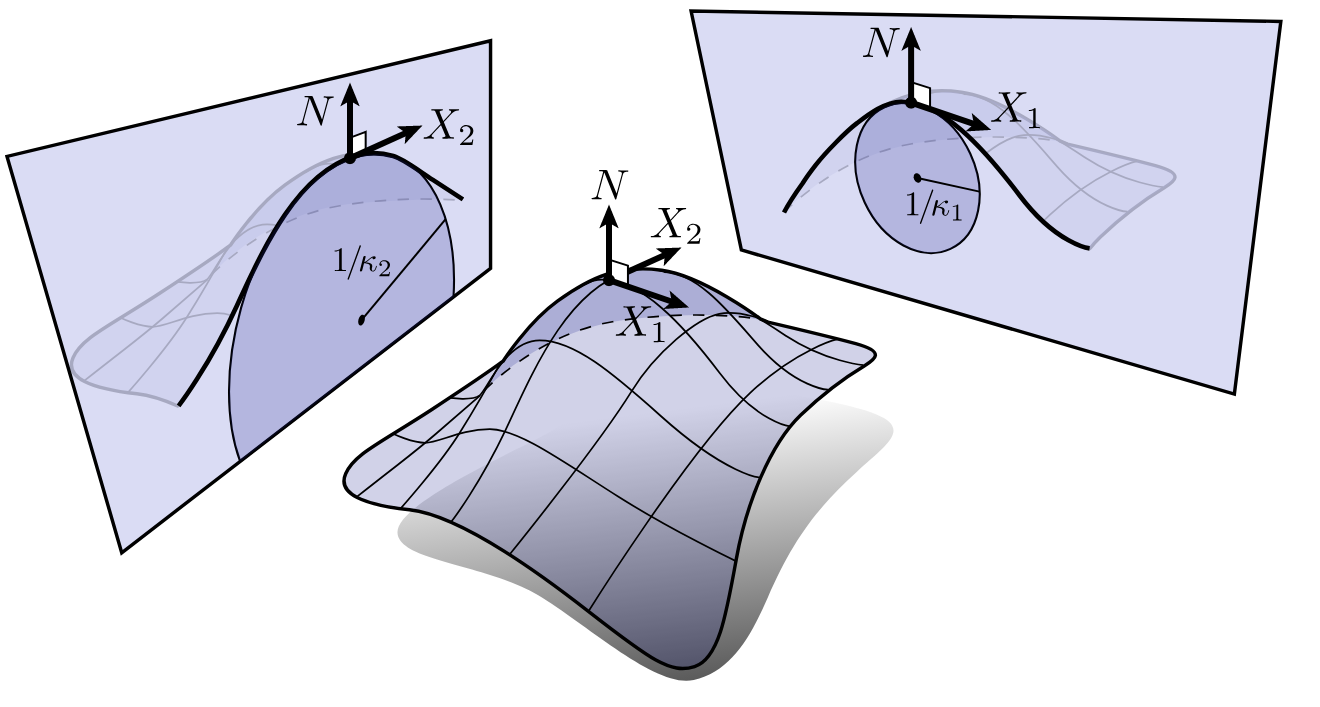
\includegraphics[width=0.7\textwidth]{img/principal}
}

\frame{{How to compute \textbf{mean curvature} on vertex?}
\begin{itemize}
  \item multiply by normal vector $\*K(\*x)=\kappa_H \*n$ %(Laplace-Beltrmi operator)
  \item $\int\int_{\mathcal{A}_M}\*K(\*x)dA=\frac{1}{2}\sum_{j\in N_1(i)}(cot\alpha_{ij}+cot\beta_{ij})(\*x_i-\*x_j)$
\end{itemize}
  \includegraphics[width=0.7\textwidth]<2>{img/star2}
  \includegraphics[width=0.7\textwidth]<3>{img/flow}
  % use barycenter if fail
  \includegraphics[width=0.3\textwidth]<4>{img/star3}\hspace{3em}
  \includegraphics[width=0.3\textwidth]<4>{img/obtuse}
}

\frame{{How to get the tensor/matrix of vertex?}
\begin{itemize}
  \item $B = \begin{pmatrix}
          a & b \\
          b & c
        \end{pmatrix}$
  \item sampling along different direction
  \item least square fitting the data constrain to mean curvature
  \item<2> $E(a,b,c) = \sum_j w_j (\mathbf{d}_{i,j}^T B \mathbf{d}_{i,j} - \kappa^N_{i,j})^2\ s.t.\ a+c=2\kappa_H, \xcancel{ac-b^2=\kappa_G}$
\end{itemize}
}

\section{problems}
\frame{{Problems}
\begin{itemize}
  \item Some pontential trouble makers
    \begin{enumerate}
     \item Hard constrain of $\kappa_H$ is replaced by soft constrain.
     \item $w_j$s are not used
     \item Area of computating $\kappa_H$ is just barycenter area, and cotangents of obtuse angles are not handled, which may cause some negative weight of summation of $\kappa_H$.
     \item \cite{meyer2003discrete} states that ``the curvature values computed from the lesast squares are often less accurate in practice''.
     \item We compute curvature of facet as the average of vertex with uniform weight
   \end{enumerate}
\end{itemize}
}

\frame{{Conclusion}
result is bad when tessellation is irregular
\begin{itemize}
  \item<3> reflection
  \item<6> burst
  \item<7> spreading
\end{itemize}
% unexpected on ground truth
  \includegraphics[width=0.6\textwidth]<2>{img/ell}
  \includegraphics[width=0.6\textwidth]<3>{img/ell2}% reflection
  \includegraphics[width=0.6\textwidth]<4>{img/ell3}
  \includegraphics[width=0.6\textwidth]<5>{img/ell4}
  \includegraphics[width=0.9\textwidth]<6>{img/cube}% burst
  \includegraphics[width=0.6\textwidth]<7>{img/cy}% spreading
}

\frame{{Ask more questions}
\begin{itemize}
\item Pipeline: $weight1 * principal\_curvature + weight2 * feature\_line \rr constrain \rr metric \rr frame\_field \rr quad$

\item<1-> How to reduce weight of bad \emph{principal\_curvature}?
\begin{enumerate}
  \item conflict with feature
  \item ``flat/sphere like'' region\\ current solution: $weight = min(|e^{|pc_1-pc_2|}-1|,100)$, still fail on the previous big triangle.
  \item other solution: subdivide or other way to change the bad tessellation.
\end{enumerate}
\item<2> what is the difference between \emph{metric} and \emph{frame\_field}?% metric is number while ff is vector?
\end{itemize}
}

\frame{{Other burst}
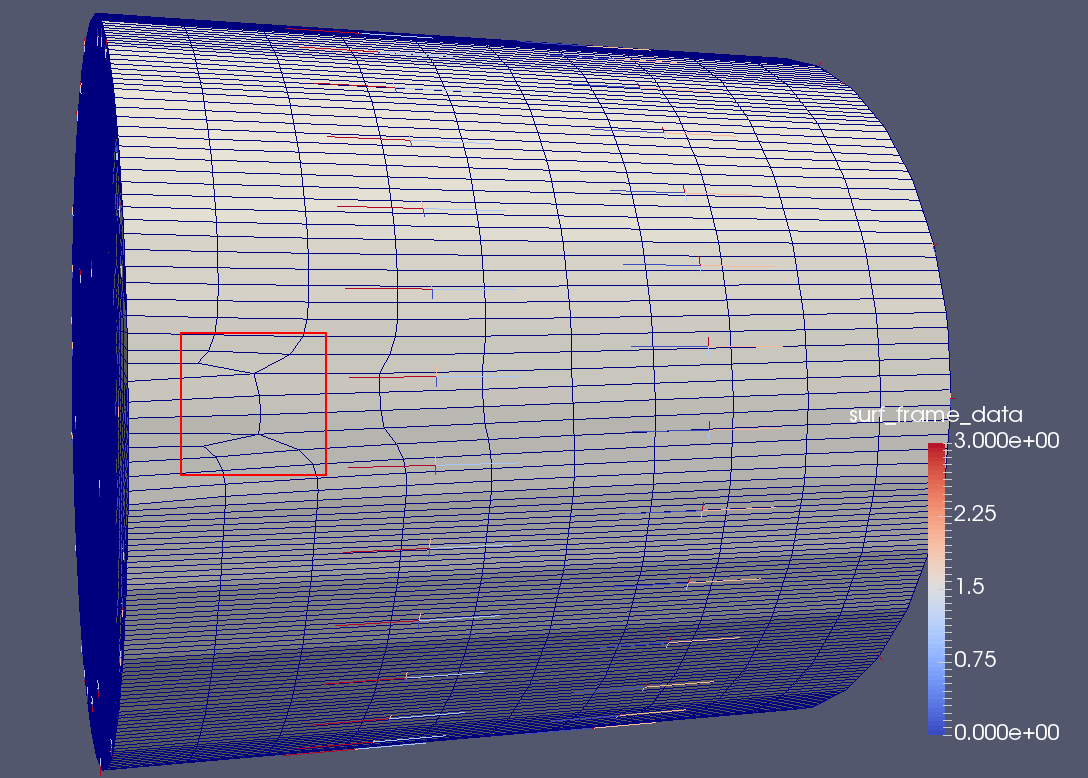
\includegraphics[width=0.6\textwidth]{img/bur}
}

\frame{{Reference}
  \bibliographystyle{amsalpha}
  \bibliography{bib}
}

\end{document}
